\section{What is the SpaceAPI?}

\begin{frame}{What is the SpaceAPI?}
	Imagine that you're travelling in a foreign country. Bored from all the
	tourist attraction, you start wondering -- are there any likeminded people
	around?

	\vspace{1em}

	\centerline{
		
\includegraphics[width=0.5\textwidth]{what_is_the_spaceapi/hacker.jpg}
	}

	So you start looking for a hackerspace, makerspace or fablab. How can you find
	out where the next such space is located?

	\vspace{1em}

	\tiny{Photo: CC BY-NC 2.0 Brian Klug}
\end{frame}

\begin{frame}{What is the SpaceAPI?}
	You found a hackerspace not too far away. There are a few things that you
	would typically want to know about that space:

	\begin{itemize}
		\item	What's the website URL of the space?
		\pause
		\item Where is the space located?
		\pause
		\item How can you contact the people from the space?
		\pause
		\item Is the space currently open?
		\pause
		\item How many people are there right now?
		\pause
		\item What projects do the people in the space work on?
		\pause
		\item How much Club Mate is still left?
	\end{itemize}

	\pause

	That's the questions the SpaceAPI tries to answer.
\end{frame}

\begin{frame}[c]{The SpaceAPI}
	The SpaceAPI is a specification for a JSON object that contains all this
	information in machine readable code.

	\vspace{1em}
	\url{http://spaceapi.net/}\\\url{https://spacedirectory.org/} (More on that later...)
	\vspace{1em}
	
\end{frame}

\begin{frame}[fragile]{Minimal Example}
	\begin{minted}[samepage=true,fontsize=\footnotesize,autogobble]{json}
{
  "api": "0.13",
  "space": "coredump",
  "url": "https://www.coredump.ch/",
  "contact": {
    "email": "vorstand@lists.coredump.ch",
    "irc": "irc://freenode.net/#coredump",
    "twitter": "@coredump_ch"
  },
  "issue_report_channels": ["email", "twitter"],
  "location": {
    "address": "Zürcherstrasse 6, 8640 Rapperswil, Switzerland",
    "lat": 47.22939, "lon": 8.82041
  },
  "logo": "https://www.coredump.ch/wp-content/uploads/2016/11/logo.png",
  "state": { "open": true, "message": "7 people present" }
}
	\end{minted}
\end{frame}

\begin{frame}[fragile]{Versioning}
Every SpaceAPI document must contain the specification version:

	\begin{minted}[samepage=true,fontsize=\footnotesize,autogobble]{javascript}
  {
    "api": "0.13",
    // ...
  }
	\end{minted}

Current version is 0.13, we're already working on the next revision. More on
that later.
\end{frame}

\begin{frame}[fragile]{General information about the space}

The space can expose information like location and contact details:

	\begin{minted}[samepage=true,fontsize=\footnotesize,autogobble]{javascript}
  {
    "space": "coredump",
    "url": "https://www.coredump.ch/",
    "contact": {
      "email": "vorstand@lists.coredump.ch",
      "irc": "irc://freenode.net/#coredump",
      "twitter": "@coredump_ch"
    },
    "location": {
      "address": "Zürcherstrasse 6, 8640 Rapperswil, Switzerland",
      "lat": 47.22939,
      "lon": 8.82041
    },
    "logo": "https://www.coredump.ch/wp-content/uploads/2016/11/logo.png",
    // ...
  }
	\end{minted}
\end{frame}

\begin{frame}[fragile]{Publish Events}

A space can publish events which happened recently and which could be
interesting to the public.

	\begin{minted}[samepage=true,fontsize=\footnotesize,autogobble]{javascript}
  {
    "events": [
      {"name": "Door", "type": "unlocked", "timestamp": 1234567},
      {"name": "Fridge", "type": "club_mate_consumed", "timestamp": 1234568},
      {"name": "Door", "type": "locked", "timestamp": 1234569},
      // ...
    ]
  }
	\end{minted}
\end{frame}

\begin{frame}[fragile]{Publish Sensor Data}

A space can publish dynamic sensor data.

	\begin{minted}[samepage=true,fontsize=\footnotesize,autogobble]{javascript}
  {
    "sensors": {
      "temperature": [
        {"location": "Soldering area", "value": 23.42, "unit": "°C"},
        {"location": "Fridge", "value": 281.78, "unit": "K"},
      ],
      "people_now_present": [
        {"location": "Hackerspace", "value": 7},
      ],
      "beverage_supply": [
        {"name": "Beer", "value": 42, "unit": "btl"},
        {"name": "Club Mate", "value": 4, "unit": "crt"},
      ],
      // ...
    }
  }
	\end{minted}
\end{frame}

\begin{frame}[fragile]{Custom Fields}
	Applications can use custom fields if they prepend the key names with ``ext\_''.

	(But often it's better to propose a new standardized field to the API.)
\end{frame}


\section{Applications}

\begin{frame}{Applications}
	If the SpaceAPI is really useful, what are some practical applications?

	We'll take a look at some of them.
\end{frame}

\begin{frame}{My Hackerspace (Android App)}
	\textit{My Hackerspace} is an Android app to check the information and status
	of any hackerspace. Select your space and start to monitor it. Available on
	F-Droid, Play Store and Github.

	\vspace{1em}
	\centerline{
		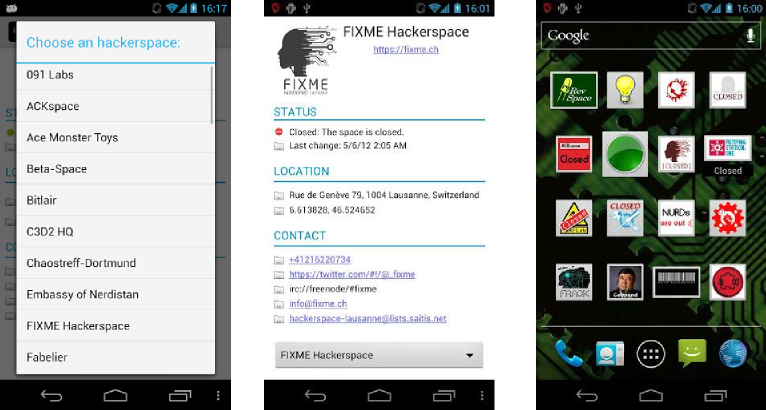
\includegraphics[width=0.75\textwidth]{what_is_the_spaceapi/app-my-hackerspace.png}
	}

\end{frame}

\begin{frame}{Space API Statistics}
	There is a website that collects historical statistics about the opening
	status of hackerspaces: \url{http://spaceapi-stats.n39.eu/}

	\vspace{1em}
	\centerline{
		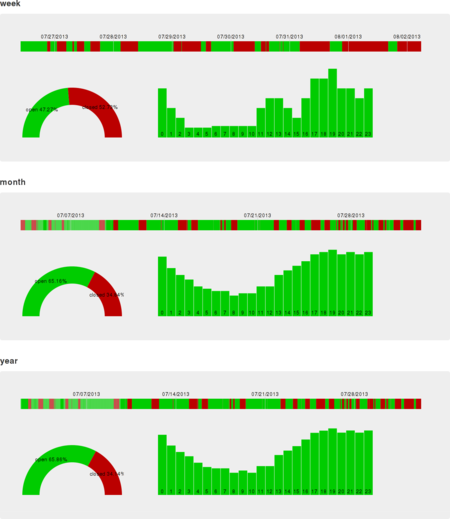
\includegraphics[width=0.75\textwidth]{what_is_the_spaceapi/app-statistics.png}
	}

\end{frame}

\begin{frame}{Spacer}
	Map of all spaces worldwide, with opening status indication:
	\url{https://spacer.nooitaf.nl/}

	\vspace{1em}
	\centerline{
		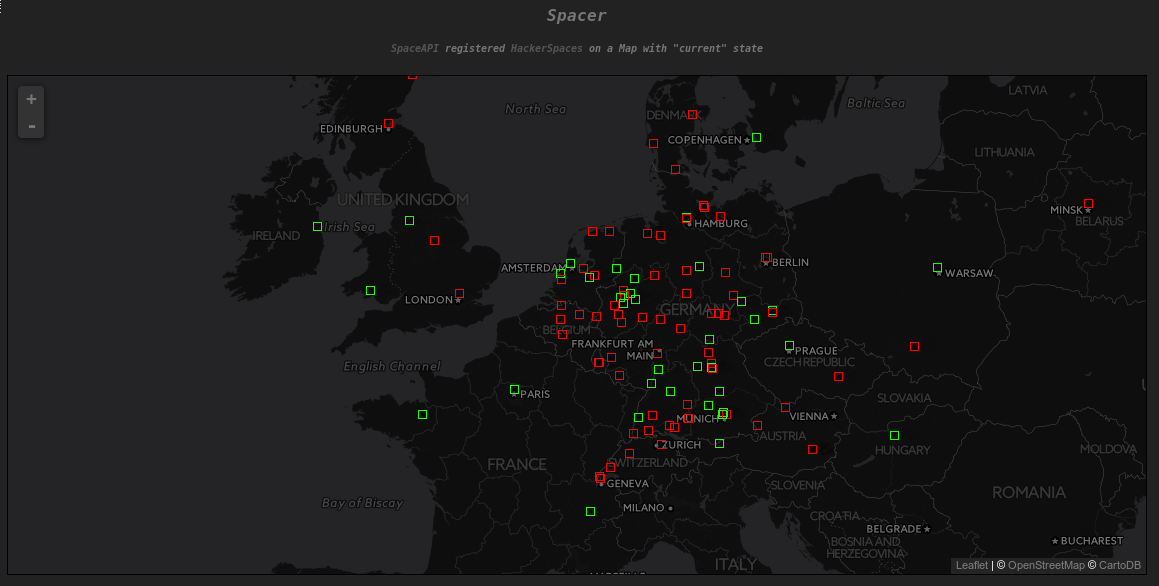
\includegraphics[width=0.9\textwidth]{what_is_the_spaceapi/app-spacer.png}
	}

\end{frame}

\begin{frame}{Wordpress Widget}
	We wrote a small Wordpress Widget that fetches the current opening status with
	JS and displays it on a website.

	\vspace{1em}
	\centerline{
		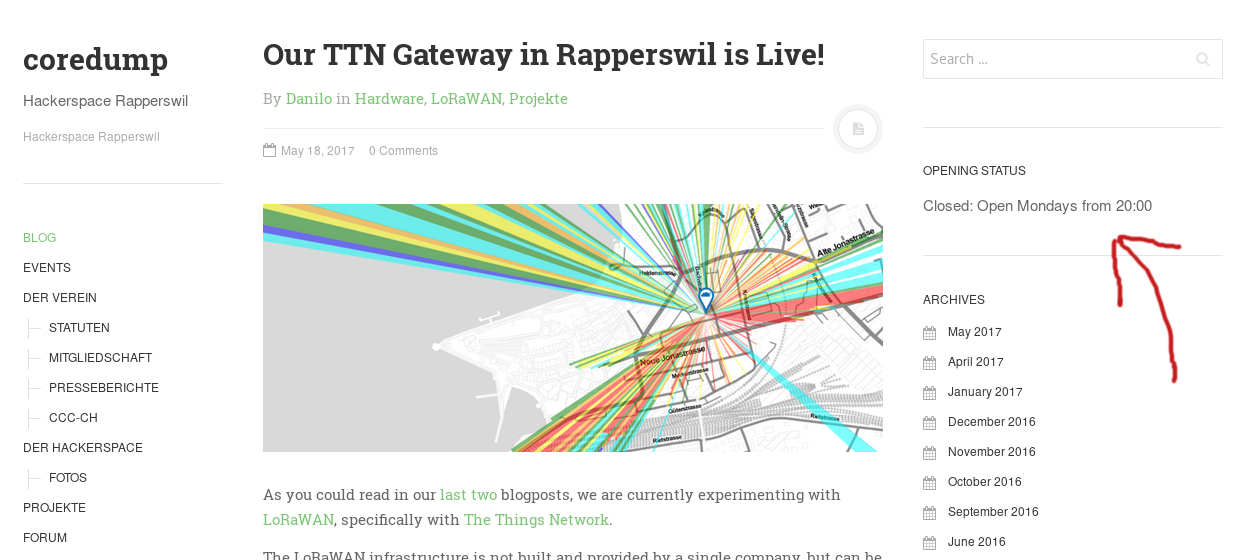
\includegraphics[width=\textwidth]{what_is_the_spaceapi/app-wp.png}
	}

\end{frame}

\begin{frame}{CCC Spaces Map}
	The CCC has created a map listing all spaces that have something like
	\texttt{"ext\_ccc": "chaostreff"} in their API response.

	\vspace{1em}
	\centerline{
		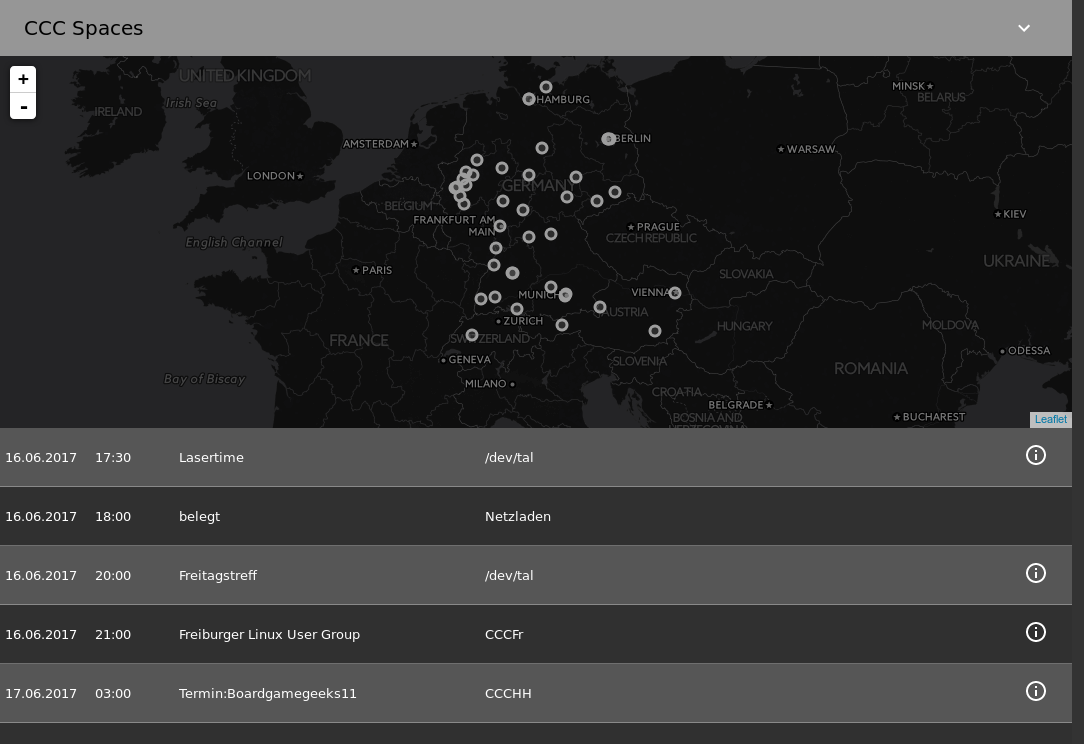
\includegraphics[width=0.9\textwidth]{what_is_the_spaceapi/app-ccc.png}
	}

\end{frame}

\begin{frame}{People Counter at Coredump}

	We wanted a way to keep track of the opening status at Coredump.
	Our solution was a binary counter to keep track of the people present, based
	on an ESP8266 board:
	
	\vspace{1em}
	\centerline{
		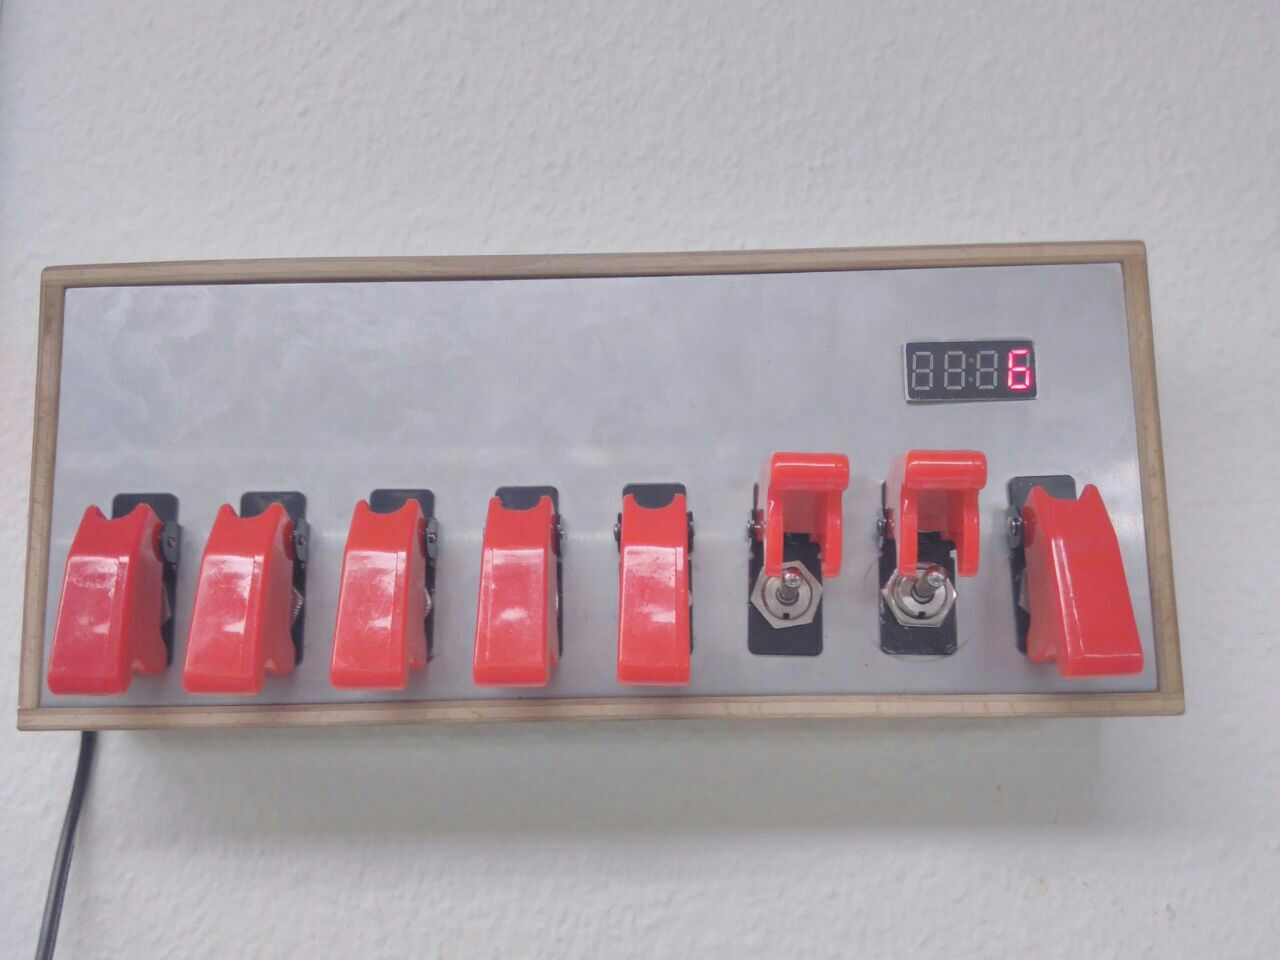
\includegraphics[width=0.6\textwidth]{what_is_the_spaceapi/counter.jpg}
	}

\end{frame}

\begin{frame}{SpaceAPI status wall at Shackspace}

	The Shackspace in Stuttgart has an awesome SpaceAPi status wall:
	
	\vspace{1em}
	\centerline{
		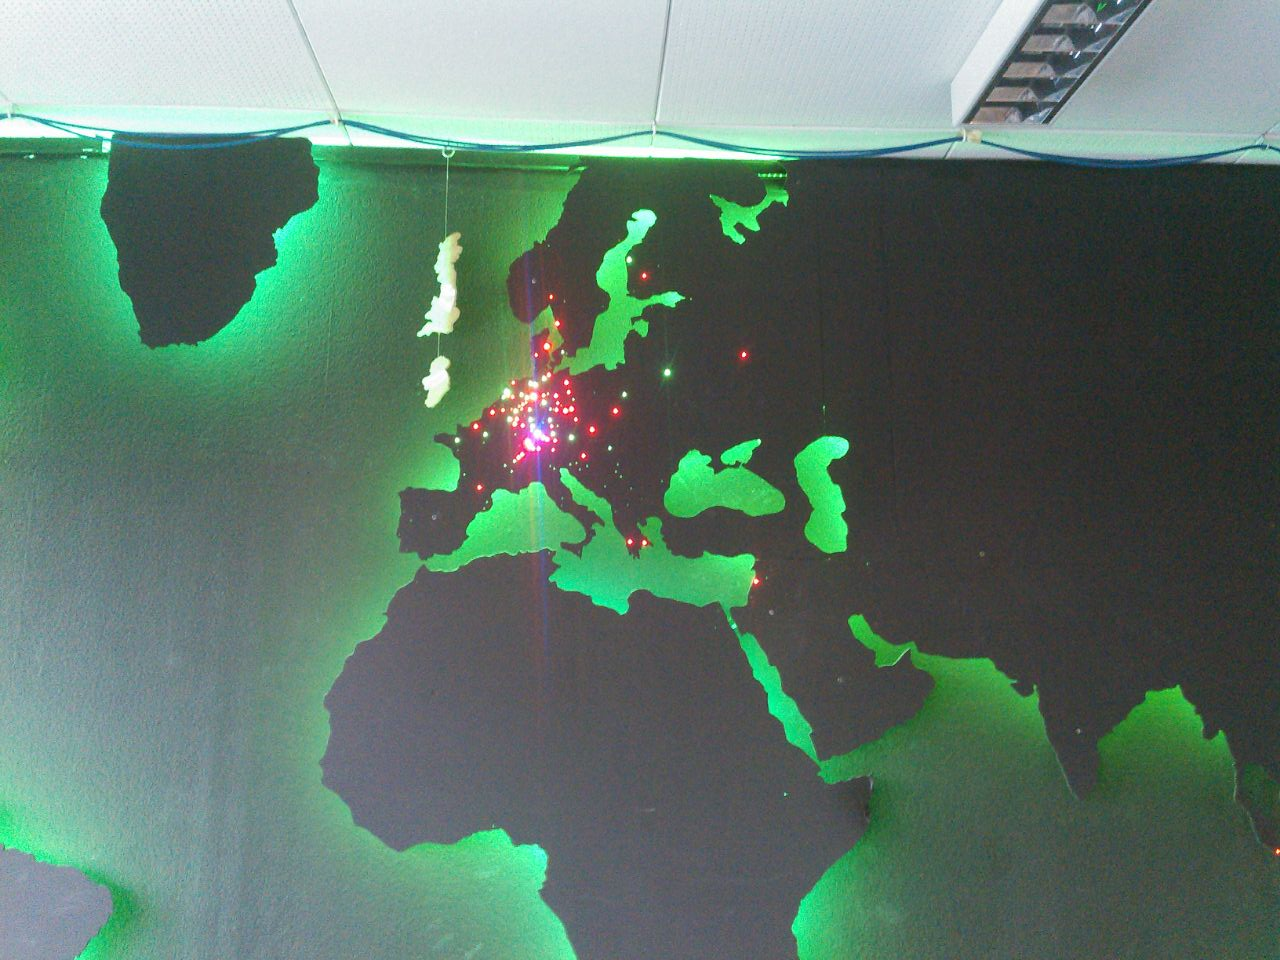
\includegraphics[width=0.6\textwidth]{what_is_the_spaceapi/statuswall.jpg}
	}

\end{frame}




\section{Implementing the SpaceAPI}

\begin{frame}{How to Implement?}
	There are a few possiblities:
	\pause
	\begin{itemize}
		\item Put a static JSON file on your webserver	
		\pause
		\item Dynamically generate a JSON file with a custom script
		\pause
		\item Create your endpoint at \url{http://spaceapi.net/new/}
		\pause
		\item Use spaceapi-server-rs (Hint: Attend our follow-up talk!)
	\end{itemize}
\end{frame}

\begin{frame}{How to Validate?}
	There's a validator at \url{http://www.spaceapi.net/validator}.

	We're writing a new one, draft of an API is at
	\url{https://validator.spacedirectory.org/}.
\end{frame}

\begin{frame}{How to Publish?}
	All SpaceAPI endpoints are collected in the Directory.

	Official directory is at \url{http://spaceapi.net/directory.json}, but it's
	often down or buggy.

	Better use directory linked at \url{https://spacedirectory.org/} instead.

	To publish your endpoint, send a pull request.
\end{frame}


\section{State of the Project}

\begin{frame}{A Little History}

	The SpaceAPI was started by @slopjong in April 2013. Right now 167 spaces are
	in the directory.

	\vspace{1em}
	\centerline{
		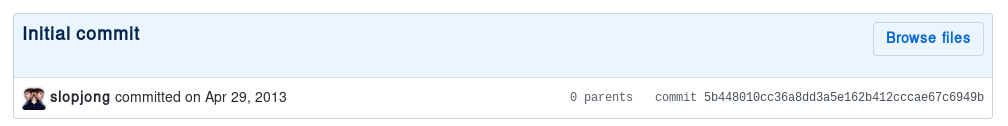
\includegraphics[width=\textwidth]{what_is_the_spaceapi/commit.png}
	}

	\pause

	Activity peaked by the end of 2013. Since then, not much has happened.

\end{frame}

\begin{frame}{A Dying Project...}
	The project didn't move forward anymore. Pull requests were left open for
	years, bugs kept appearing.

	We contacted the maintainer of the project to ask whether we could help, but
	he's very busy with other projects and we couldn't find a way to get more
	maintainers into the project.
\end{frame}

\begin{frame}{...and a Revival!}
	So at the CCC Congress 2016 we friendly-forked the project and created the
	\url{spacedirectory.org} website.

	\vspace{2em}
	\centerline{
		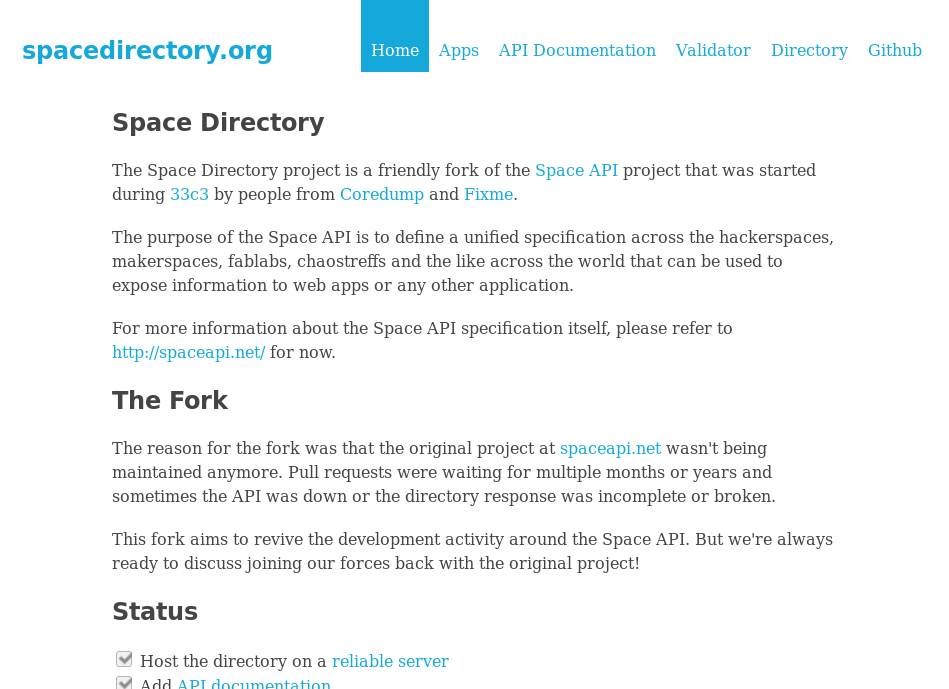
\includegraphics[width=0.9\textwidth]{what_is_the_spaceapi/spacedirectory.png}
	}
\end{frame}

\begin{frame}{Current Status}
	\begin{itemize}
		\item \checkmarkbox Host the directory on a reliable server
			\pause
		\item \checkmarkbox Add API documentation
			\pause
		\item \checkmarkbox Port JSON schema files to new format (IETF draft 4)
			\pause
		\item \checkmarkbox Create updated apps page that showcases existing projects
			\pause
		\item \emptybox Write a simple schema validator (work in progress)
			\pause
		\item \emptybox Add a "getting started" guide to the website (planning)
			\pause
		\item \emptybox Maybe rewrite the directory server (planning)
	\end{itemize}
\end{frame}

\begin{frame}{The Future}
	Some things are happening, maybe we can join back with the original SpaceAPI.

	In any case, implement the API, help improving the Space Directory or hack on
	our Rust SpaceAPI implementation!

	\vspace{4em}

	\centerline{\huge \url{spacedirectory.org}}
\end{frame}

\section{Questions?}
